\chapter{GPGPU - Obecné výpočty na grafické kartě}  \label{sec:gpgpu}
Obecné výpočty na grafické kartě (anglicky General-Purpose computing on graphics processing unit, zkratka GPGPU) využívají výpočetní síly grafických procesorů, které byly původně navrženy pouze pro výpočty v počítačové grafice. Ve spolupráci s CPU jsou ale v tomto případě využívány k řešení obecných úloh, které jsou normálně zpracovávány pouze CPU.\\

Protože řešení grafických úloh vyžaduje většinou mnoho vektorových a maticových výpočtů, které jsou mnohdy snadno paralelizovatelné, obsahuje architektura GPU mnoho jednoduchých výpočetních jader schopných počítat základní matematické operace a pracovat paralelně. Jejich hlavní výhodou oproti běžným CPU, je tady fakt, že obsahují stokrát, v poslední době až tisíckrát, více jader navržených k paralelním výpočtům, takže pokud je úloha dobře paralelizovatelná a vyžaduje pouze jednoduché matematické úlohy, můžeme její výpočet urychlit až tisícinásobně v porovnání s CPU.\\

Z počátku podporovaly grafické karty pouze vektorové a maticové výpočty s dimenzí 2, 3 nebo 4, protože se tyto struktury běžně používají v grafických výpočtech. Pokud jsme tedy chtěli počítat běžné úlohy, bylo potřeba je přeformulovat a složit pouze z grafických operací podporovaných grafickými rozhraními jako je DirectX či OpenGL. Tato transformace byla pro programátory velmi náročná a často dokonce nemožná, takže mnoho algoritmů nemohlo výpočetní potenciál grafických karet využít.\\

Tento problém ale zmizel s příchodem specializovaných nástrojů pro využití GPU pro obecné výpočty. Tyto frameworky umožňují vývojářům oprostit se od limitací daných grafickým prostředím a využít GPU k obecným výpočtům mnohem jednodušeji.~\cite{Kirk12}\\

V dnešní době existují 2 hlavní frameworky pro GPGPU, konkrétně CUDA~\cite{Sanders10} a OpenCL~\cite{Scarpino11} (open computing language). CUDA má oproti konkurenčnímu OpenCL velkou výhodu v přímé vazbě na hardware. Je to dáno tím, že CUDA je vyvíjena firmou Nvidia pouze pro vlastní karty, takže může využívat specifických vlastností konkrétní architektury. V porovnání s tím je OpenCL od skupiny Khronos univerzální nezávislý framework pro paralelní výpočty podporující široké spektrum výpočetních čipů, které se mohou architektonicky velice lišit. OpenCL lze tedy zprovoznit jak na GPU včetně karet od Nvidia, tak na běžných CPU. Tato podpora je ale problematická pokud chceme vysoký výkon, protože OpenCL nemůže využívat všech vlastností konkrétní architektury a hardware jednoduše proto, protože zde neexistuje žádná konkrétní architektura. V této práci jsme se tedy rozhodli využít frameworku CUDA, protože nám nejde o podporu co nejvíce zařízení, ale chceme se naopak zaměřit na co nejlepší optimalizaci. Další výhodou CUDA je, že kód, který běží na CPU a kód, který běží na GPU, jsou psány společně a jsou oba kompilované při sestavování kódu, v čemž se liší od OpenCL, kde se kód pro GPU kompiluje až při běhu.

\section{Architektura GPU}
GPU je multiprocesor vysoce vyladěný pro grafické výpočty, které vyžadují rychlé zpracování velkého množství operací s plovoucí desetinou čárkou. Fyzicky bývá GPU umístěn na dedikované kartě připojené k základní desce pomocí sběrnice PCI Express nebo může být přímo součástí procesorového čipu. Protože integrované GPU nejsou příliš výkoné, zaměříme se především na externí grafické karty, na které bývá kromě samotného grafického procesoru i paměť, která slouží ke zmenšení latence. GPU se běžně skládá z těchto komponent:
\begin{description}
\item[unifikované shadery] jsou programovatelné výkonné jednotky zodpovědné za výpočty. Historicky nahradily specializované shadery jako například vertex shadery nebo pixel shadery. Díky unifikaci tak můžeme lépe rozložit výpočetní zátěž a například pro úlohy s mnoha geometrickými operacemi pak může systém využít většinu shaderů pro geometry shadery. Díky unifikovaným shaderům jsme také schopni počítat na GPU obecné výpočty.
\item[paměťový řadič] je zodpovědný za komunikaci mezi CPU a grafickou pamětí.
\item[jednotka pro mapování textur] umisťuje jednotlivé textury na objekty.
\item[vykreslovací jednotka] vytváří výsledný obraz a posílá ho na výstupní zařízení.
\end{description}

Pro GPGPU výpočty se tedy využívají pouze unifikované shadery a paměť s paměťovým řadičem.

\subsection{Porovnání GPU a CPU} \label{ssec:gpucpucomparison}
Hlavním rozdílem mezi CPU a GPU je jejich specializaci. Na rozdíl od obecného zaměření CPU se GPU specializuje na grafické výpočty. Ty vyžadují vysokou propustnost dat, takže je jejich architektura zaměřena na masivně paralelní výpočty s čísly. Jednotlivá jádra se také liší. CPU jádro běžně pracuje na vyšší frekvenci (2 - 4 GHz) a podporuje mnoho instrukcí. Oproti tomu jádro GPU je taktované na nižší frekvenci (0,8 - 1 MHz) a podporuje pouze speciální množinu instrukcí. Dříve se tedy nebylo potřeba tyto 2 jednotky vůbec porovnávat, protože se zaobíraly zcela jinými problémy, ale s příchodem GPGPU si začaly konkurovat. Hlavní rozdíly mezi CPU a GPU jsou tyto:
\begin{description}
\item[Počet jader] CPU má pouze pár fyzických jader~\autoref{fig:cpuarchitecture}, běžné CPU mezi 2-8 jádry, serverové pak mezi 8 až 16 jádry na jednom čipu. V porovnání s tím má moderní GPU kolem 1000 CUDA jader~\autoref{fig:gpuarchitecture},nejlepší modely mají pak tisíce jader(například, GeForce GTX Titan Xp má 3 840 CUDA jader), takže mají obrovský potenciál pro paralelní výpočty.
\item[architektura jádra] jádra GPU jsou specializované na numerické výpočty, nikoliv na obecné úlohy jako je tomu u CPU jader. Tím ale nejsou nijak limitovány, protože jsou většinou využívány právě k numerickým výpočtům. Výhodou CPU je frekvence, která se většinou pohybuje okolo pětinásobku frekvence GPU jádra. Díky optimalizacím GPU jader na numerické úkoly jsou tato jádra schopna spočítat rychleji než běžné CPU a frekvence tak není tolik limitující. Nižší frekvence GPU jader má více důvodů. Problematický je například odvod velkého množství tepla vyrobeného tisíci jader na jediném čipu. Protože vyšší frekvence znamená i více vygenerovaného tepla, nemohou jádra GPU běžet na takové frekvenci jako jádra CPU.
\item[Vlákna] Přístup k vláknům se také liší. CPU je schopno zpracovat více instrukcí v jednom okamžiku, což je označováno jako Simultaneous Multithreading (SMT), GPU multiprocesor umožňuje běh více vláken najednou, ale jednotlivá vlákna vykonávají stejný kód, protože výpočetní jednotky sdílí jednotku pro čtení a dekódování instrukcí (fetch/decode unit).
\item[Paměť] CPU má velkou cache paměť, pomocí které řeší latenci při přístupu k datům. Pokud je tedy vlákno přesunuto na jiné jádro, lokálně cachovaná data mohou být nepoužitelná (v závislosti na typu cache) a nové jádro si musí data znovu nacachovat. GPU má oproti tomu pouze menší cache, ale vlákna se za běhu mezi vlákny nepřesouvají.
\end{description}

\begin{figure}[h]
\centering
\begin{subfigure}{.49\textwidth}
  \centering
  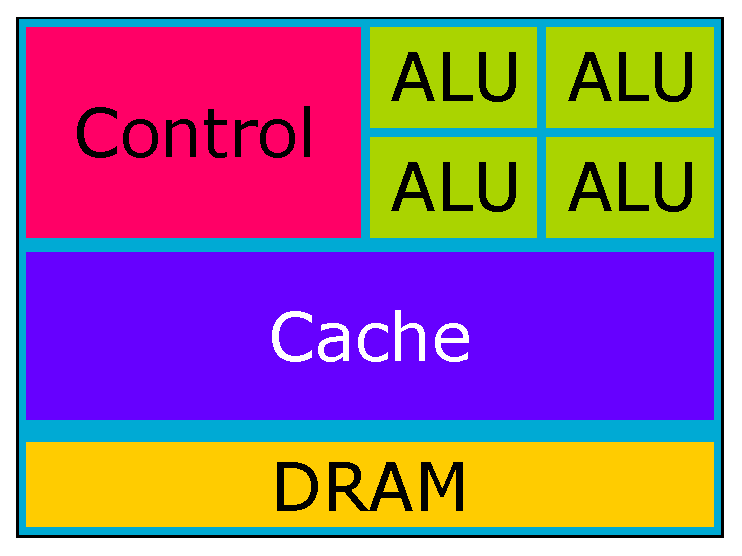
\includegraphics[width=1\linewidth]{img/CPUarchitecture.eps}
  \caption{architektura CPU}
  \label{fig:cpuarchitecture}
\end{subfigure}
\begin{subfigure}{.49\textwidth}
  \centering
  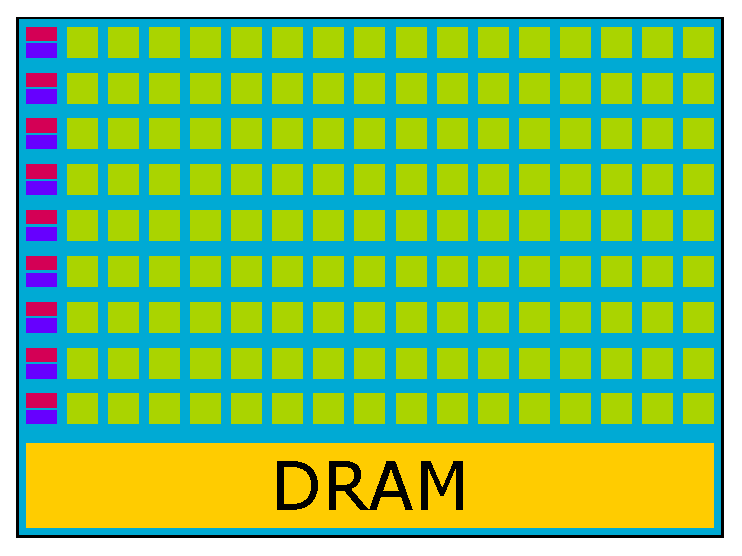
\includegraphics[width=1\linewidth]{img/GPUarchitecture.eps}
  \caption{architektura GPU}
  \label{fig:gpuarchitecture}
\end{subfigure}
\caption{Porovnání architektury CPU a GPU (stejné barvy obdélníku znamenají stejné jendotky)}
\end{figure}

%\begin{table}
%\begin{tabular}{|l|l|l|}
%\cline{1-2}
%NIC & CPU & GPU \\ \cline{1-2}
%# cores & Few cores per chip & Many cores per chip \\ \cline{1-2}
%Specialization & General purpose cores & Cores psecialized for numeric computations \\ \cline{1-2}
%Threads approach & Processing different threads & SIMT thread processing \\ \cline{1-2}
%Memory access & Huge caches to reduce memory latency & Huge amount of threads and fast context switch \\ \cline{1-2}
%\end{tabular}
%\end{table}
\section{CUDA}
CUDA (Compute Unified Device Architecture) je platforma pro paralelní výpočty pro GPGPU vyvíjená společností Nvidia. Zahrnuje jak hardwarovou tak softwarovou architekturu integrovanou na grafických kartách Nvidia. CUDA podporuje více programovacích jazyků, konkrétně C, C++ a Fortran, což ji dělá přístupnější pro vývojáře. Existují i jiné platformy, jako například OpenCL, ale z důvodů popsaných výše se jimi nebudeme zabývat.\\

\begin{figure}[h]
\centering
%\begin{subfigure}{0.49\textwidth}
%  \centering
%  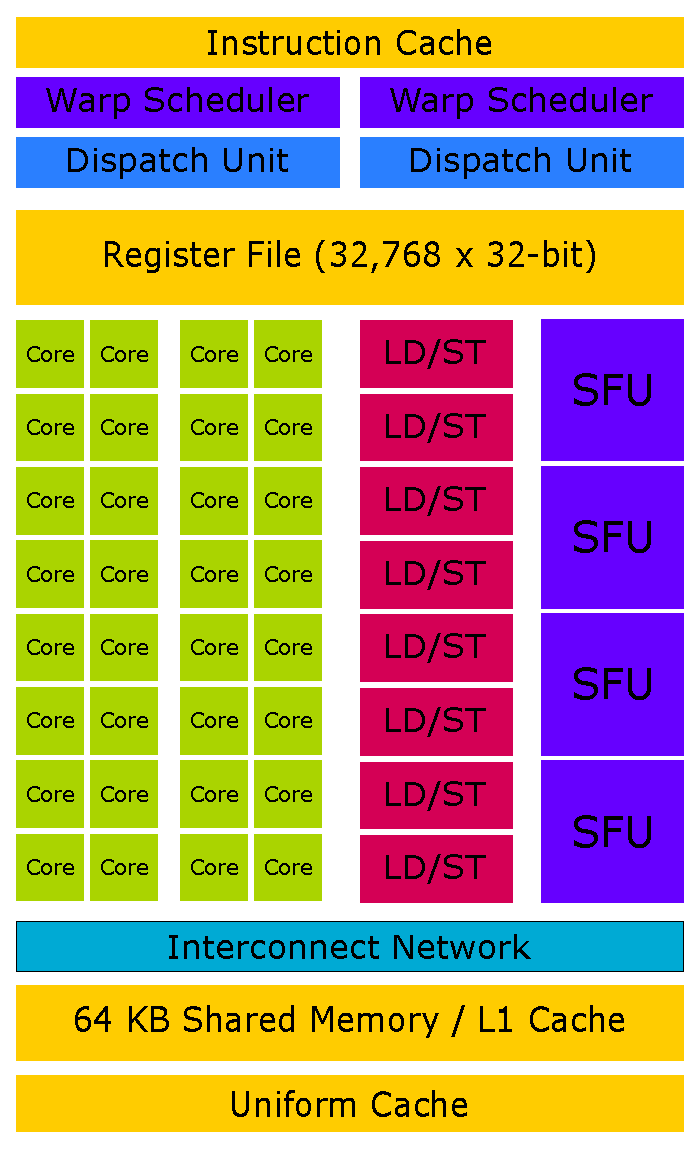
\includegraphics[width=0.8\linewidth]{img/SMPArchitecture.eps}
%  \caption{SMP architecture (Fermi)}
%  \label{fig:smparchitecture}
%\end{subfigure}
%\begin{subfigure}{0.6\textwidth}
  %\centering
  %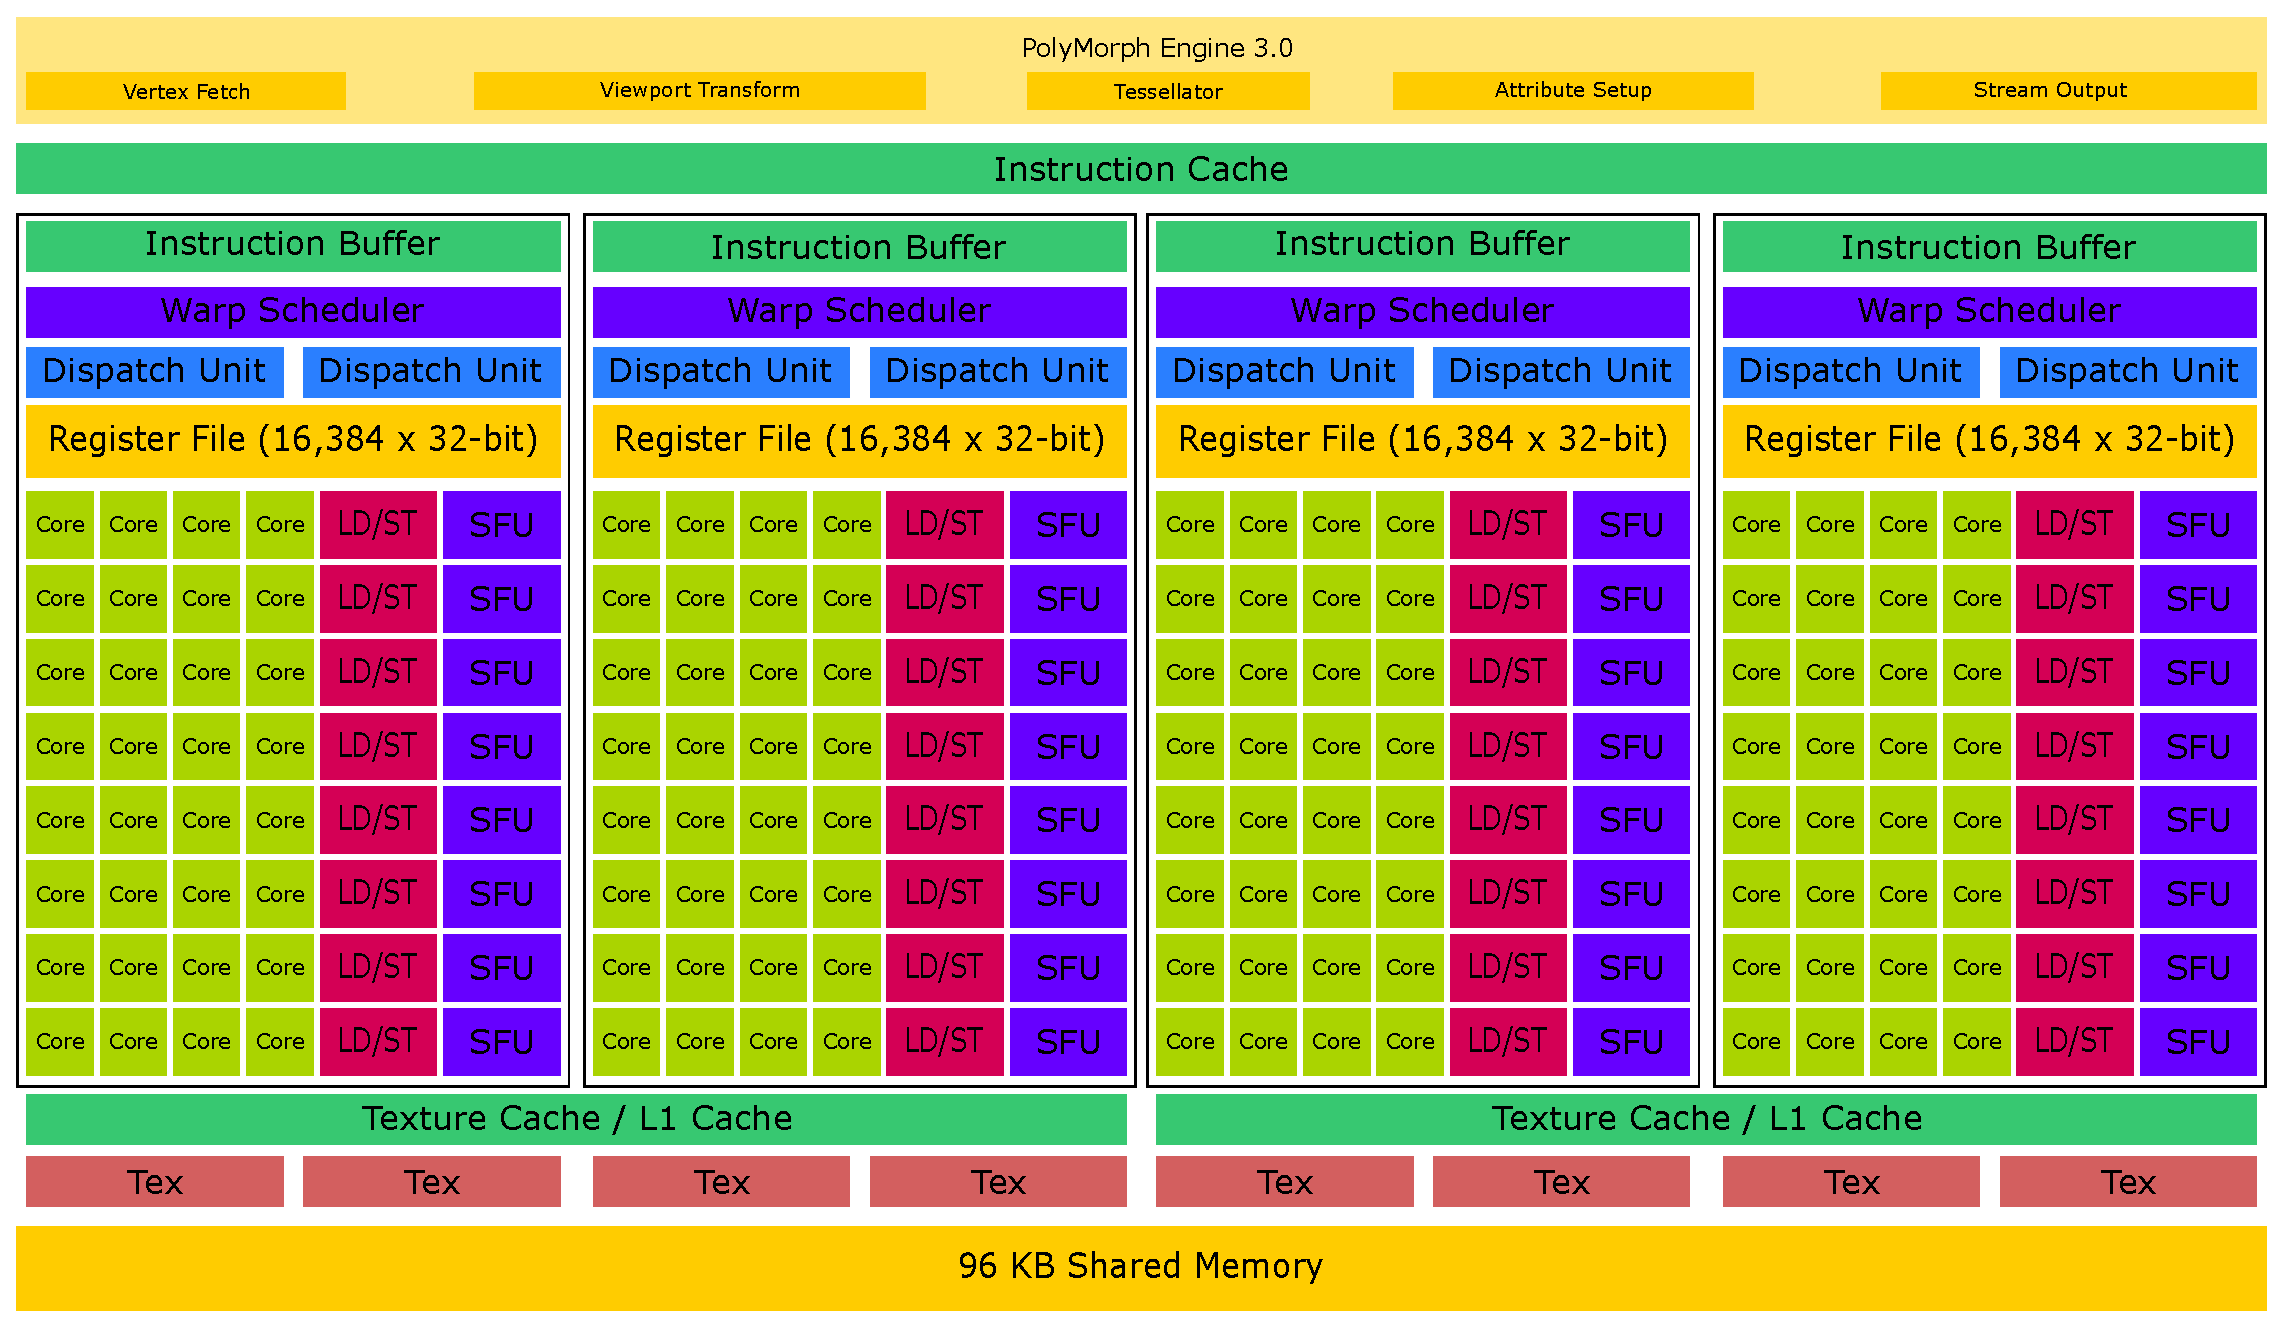
\includegraphics[width=1\linewidth]{img/SMMArchitecture.eps}
  %\caption{Architektura SMM (Maxwell)}
 % \label{fig:smmarchitecture}
  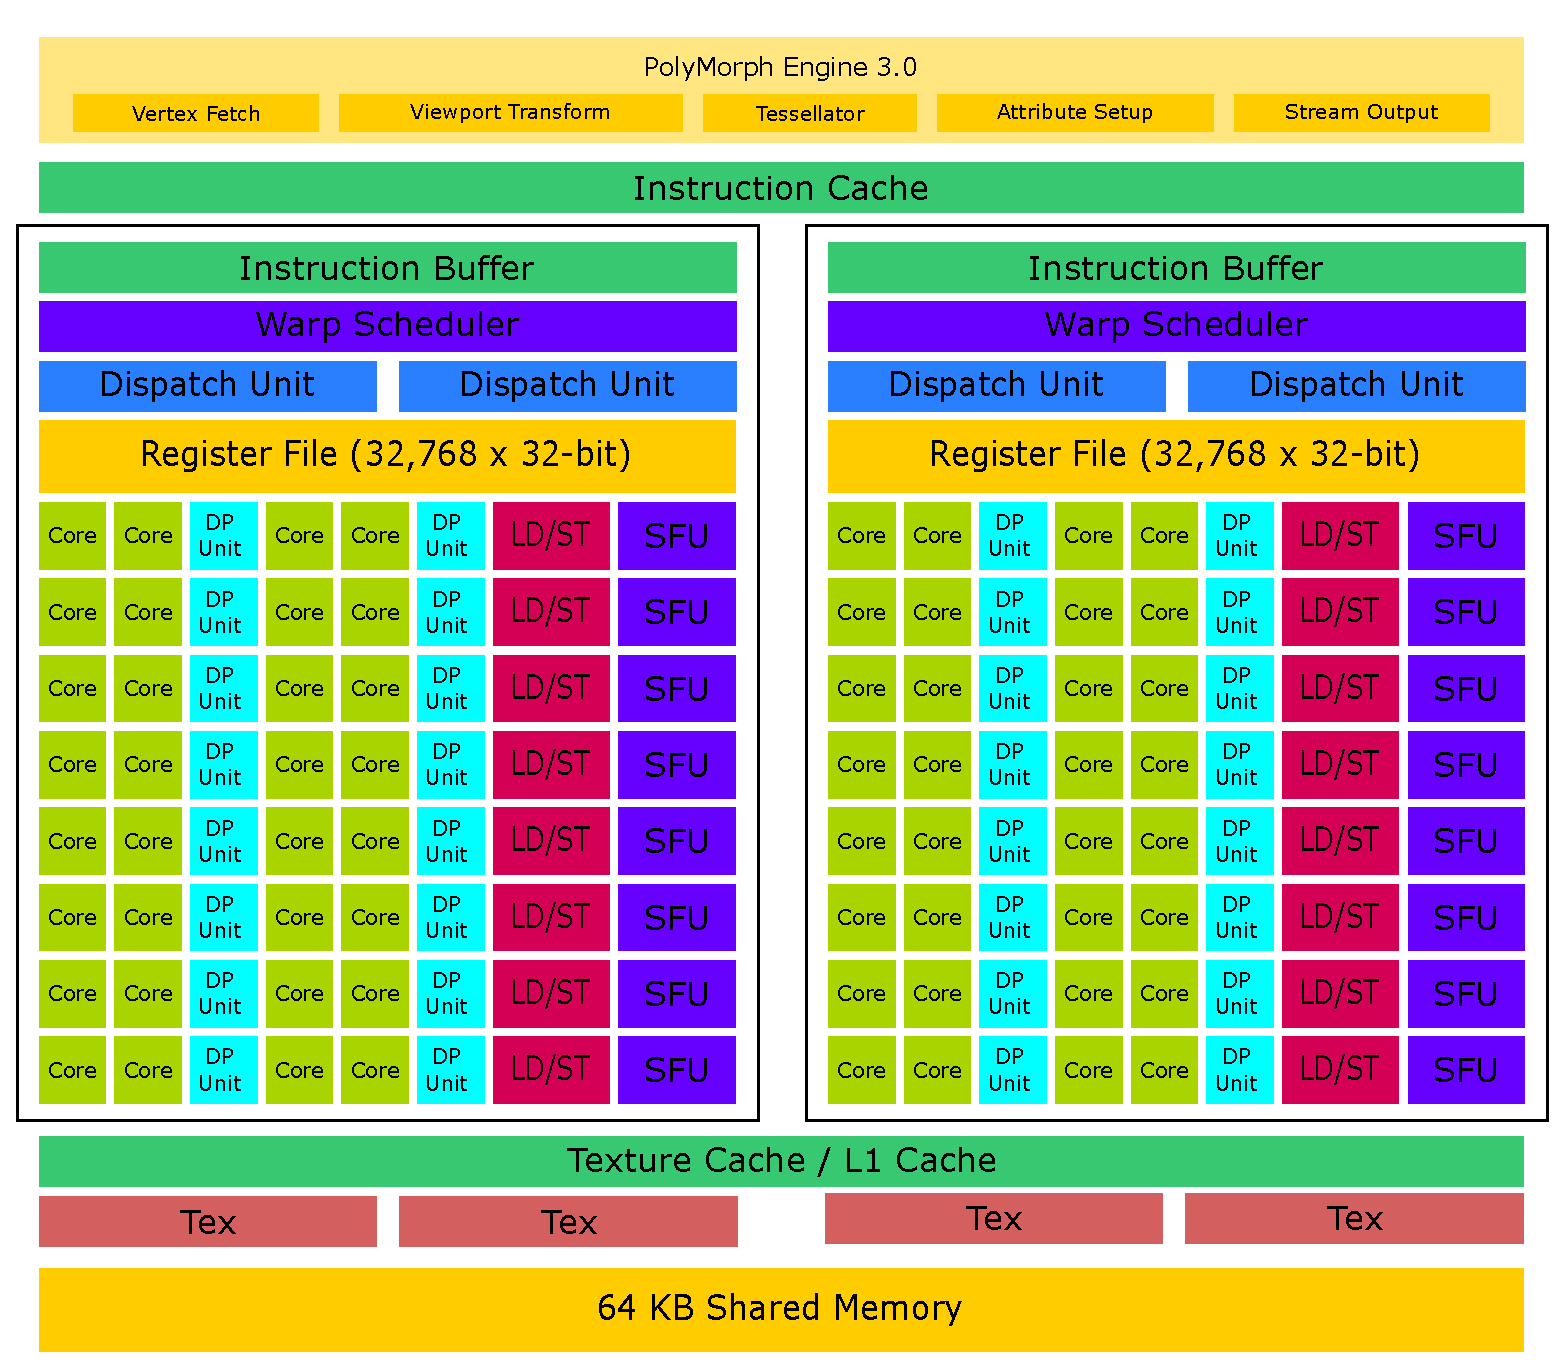
\includegraphics[width=1.0\linewidth]{img/PSMArchitecture.eps}
  \caption{Architektura PSM (Pascal)}
  \label{fig:psmarchitecture}
%\end{subfigure}
%\vspace*{0.1cm} 
%\begin{subfigure}{0.6\textwidth}
%  \centering
%  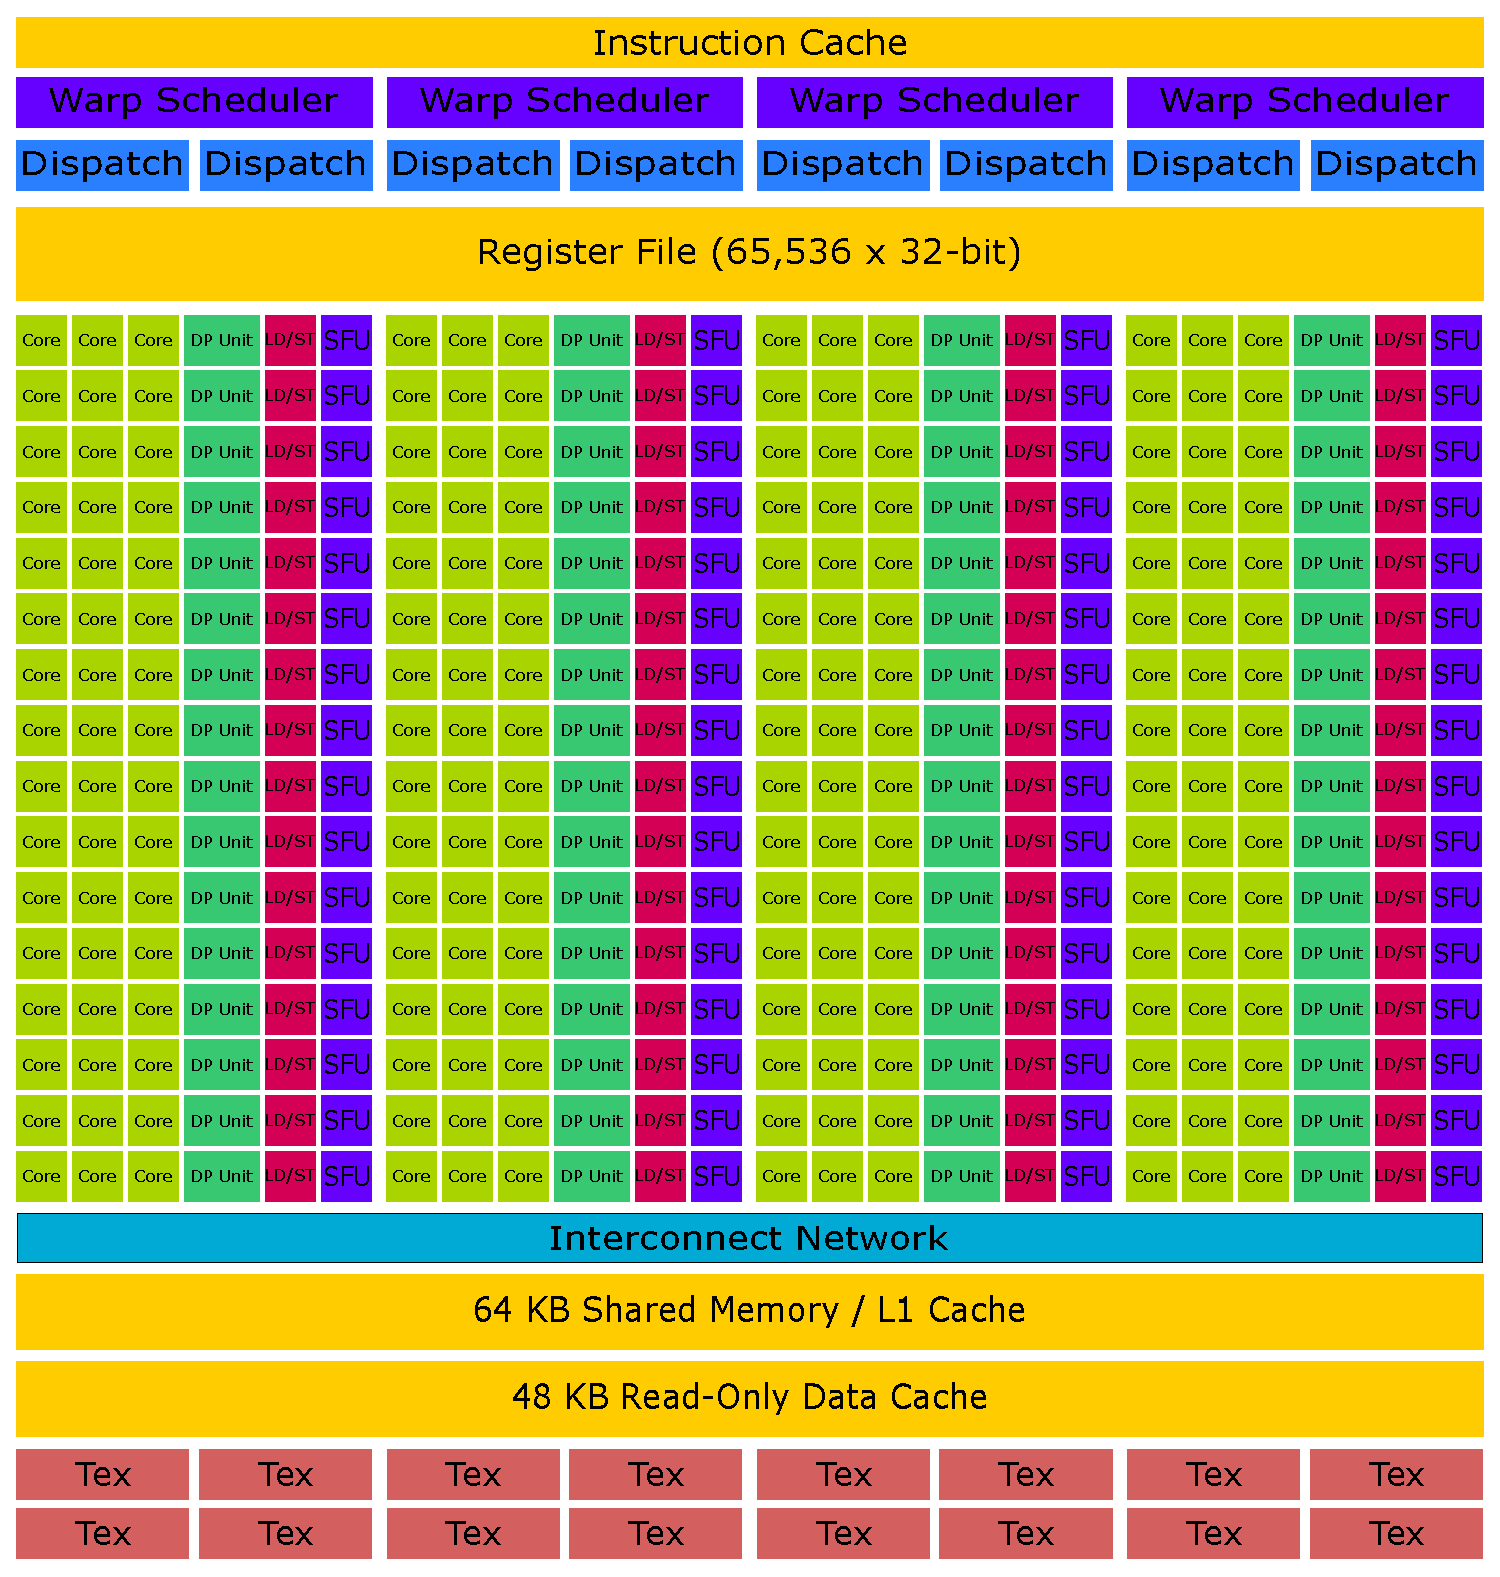
\includegraphics[width=0.9\linewidth]{img/SMXArchitecture.eps}
%  \caption{SMX architecture (Kepler)}
%  \label{fig:smxarchitecture}
%\end{subfigure}
\end{figure}

CUDA architektura obsahuje více větších procesorů zvaných \textbf{Streaming Multiprocessor (SMP)}. Nejstarší generací je \textbf{SM} - Fermi, následuje \textbf{SMX} - Kepler, novější \textbf{SMM} - Maxwell a nejnovější \textbf{PSM} - Pascal~\autoref{fig:psmarchitecture}. Každý SMP obsahuje výpočetní jádra s registry (32 na architektuře Fermi, 64 na architektuře Pascal, 128 na architektuře Maxwell a 192 na architektuře Kepler), načitací a zápisové jednotky (load/store - LD/ST), jednotky pro speciální funkce (SFU), sdílenou instrukční cache, sdílenou paměť (shared memory) a datovou cache (data cache). LD/ST a SFU jednotky jsou sdíleny skupinami jader. Velikost těchto skupin závisí na konkrétní architektuře. Architektura Pascal navíc obsahuje ke každým 2 jednotkám pro single floating point operace ještě jednu double floating ponint jednotku (DP).\\

\begin{figure}[h]
  \centering
  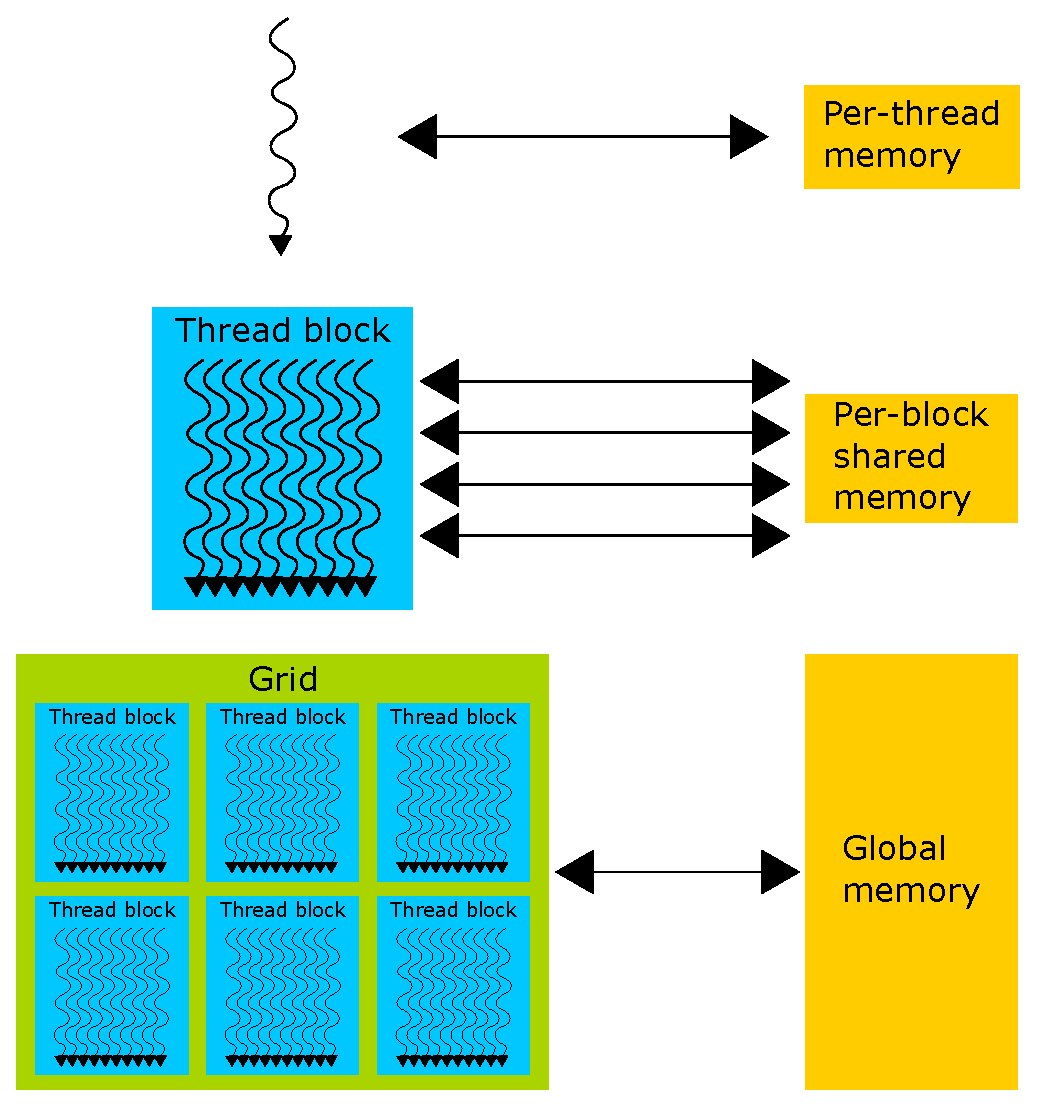
\includegraphics[width=0.8\linewidth]{img/CUDAmemoryHierarchy.eps}
  \caption{Výpočetní model CUDA}
  \label{fig:cudamemhierarchy}
\end{figure}

Dalším parametrem odlišující jednotlivé CUDA zařízení je \textbf{Compute Capability} (CC), která udává vlastnosti zařízení a sadu instrukcí, které jsou podporované. CC je úzce spjatá s architekturou(CC 1.x byla podporována architekturou Tesla, CC 2.x na Fermi, 3.x na Kepleru, 5.x na Maxwellu a 6.x na Pascalu).\\

CUDA využívá modelu Simple Instruction Multiple Thread (SIMT). Tento model přistupuje k paralelizaci tak, že je jedna instrukce vykonávána více výpočetními jednotkami, takže stačí pouze jedna fetch/decode jednotka pro načítání instrukcí pro celou skupinu výpočetních jednotek. Tento model je podobný modelu Simple Instruction Multiple Data (SIMD), ale rozdíl je v tom, že SIMT má více registrů. SIMD jednoduše zpracovává malé vektory paralelně a všechna vlákna dělají tu samou operaci. Pokud tedy chceme například sešíst 2 vektory, SIMD musí iterovat přes celý vektor a v každém kroku může zpracovat tolik prvků, kolik má výpočetních jednotek.Oproti tomu CUDA se SIMT modelem může nastartovat tolik vláken, jako je velikost vektoru a každé vlákno si pak výsledek uloží ve svém registru.\\

\subsection{CUDA Workflow}
When we want to launch CUDA program, first think what we must do in host code is detect CUDA capable devices. When desired device is selected, we could start with copying data from host to device. This action is asynchronous so we must synchronize execution of host code and memory transfer. When data transfer is done, we could launch device code called \textbf{kernel}. Kernel is same as normal C function but defined with special declaration and it can use special device functions specified by CC. \\
Kernel is launched from host code same as normal function but it runs asynchronously. This function is executed $N$ times in parallel by different CUDA threads. Number of threads is specified at function call. Threads are arranged in one, two or three dimensional space so it could easily reflect data structures like vectors, matrices or volumes. This bunch of threads is called \textbf{block}. The number of threads in block is limited because all threads in block must reside on the same streaming multiprocessor and must share its limited memory resources so on current GPUs, maximum number of threads is 1024.\\
The total number of threads is multiplied by number of blocks. Blocks could be also arranged in one, two or three dimensional space. Only limitation is that each block must be equally shaped so usually the number of thread blocks is determined by size of data being processed or by total number of cores. The total number of threads which are executed in single kernel is number of threads times number of blocks as specified on~\ref{fig:cudagridthreadblock}. Kernel is also called asynchronously so when kernel is executing, host could for example start another memory transfer or doing another work on CPU. After synchronizing with device, we need usually transfer results from the device back to host which is again asynchronous call and must be synchronized.

\begin{figure}[h]
  \centering
  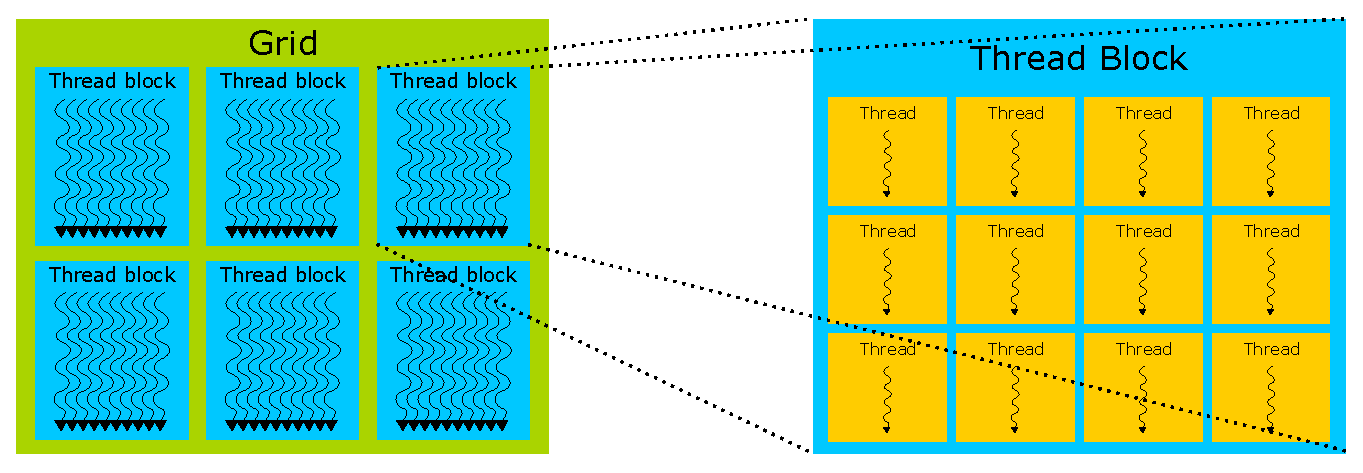
\includegraphics[width=1\linewidth]{img/CUDAthreadGridBlock.eps}
  \caption{2-dimensional grid of 2-dimensional thread blocks}
  \label{fig:cudagridthreadblock}
\end{figure}

Because number of cores is usually smaller than number of threads specified on kernel launch, only some threads could be run in parallel. These groups of threads are called \textbf{Warps}. When Kernel is launched, each block is assigned to SM and does not migrate to another SMP. Than, Each SMP splits its blocks into Warps depends on architecture. Warp threads are executed simultaneously by SMP cores. Splitting of the work between blocks and threads could significantly change the performance, because when we choose bad size of block (indivisible by Warp size) some Warps will not use all cores of single SMP. for example, if we launch same kernel with 8 blocks of 96 threads, block will be split into 3 warps which will be executed in parallel so we will have 24 warps to compute. Compare to that, if we launch the same kernel with 64 blocks of 12 threads, each block will be represented by warp containing only 12 threads so the total number of warps for execution will be 64 because CUDA is not capable to coalesce threads from different blocks. For this reason, it is recommended to set the size of the block to number divisible by size of Warp.\\
There are limitations for operations which could be run in parallel. For example, on Kepler architecture, only 4 of the 12 groups of cores can execute double precision operations at one time, so the slowdown of double precision computation may be up to 3 times. However, the other 8 groups could perform integer or float operations so the slowdown is usually smaller.\\
Problematic are problems with memory operations. Common CPU hides these latency by multilevel cache memory. CUDA architecture also contains some memory caches~\ref{fig:cudamemhierarchy} but because of the most common specialization of algorithms accelerated on GPU - stream or throughput computing, memory caching is ineffective. On CUDA, this is problem is reduced by more active warps on one core so when one warp stalls on memory operation, SMP switches to another ready warp. This mechanism keeps computing cores busy as possible and increasing the efficiency of computation.\\
Threads in single block are executed on a single SM. They share caches and could be synchronized across the threads from same warp. Compared to that threads from different Thread Blocks could be assigned to different SMPs or on same SMP concurrently. They could be even assigned to different or same SM at different times.

\subsection{Memory model}

Memory model on CUDA architecture~\ref{fig:cudamemaccess} contains more types of memory which differs mainly in size, bandwidth and latency.

\begin{figure}[h]
  \centering
  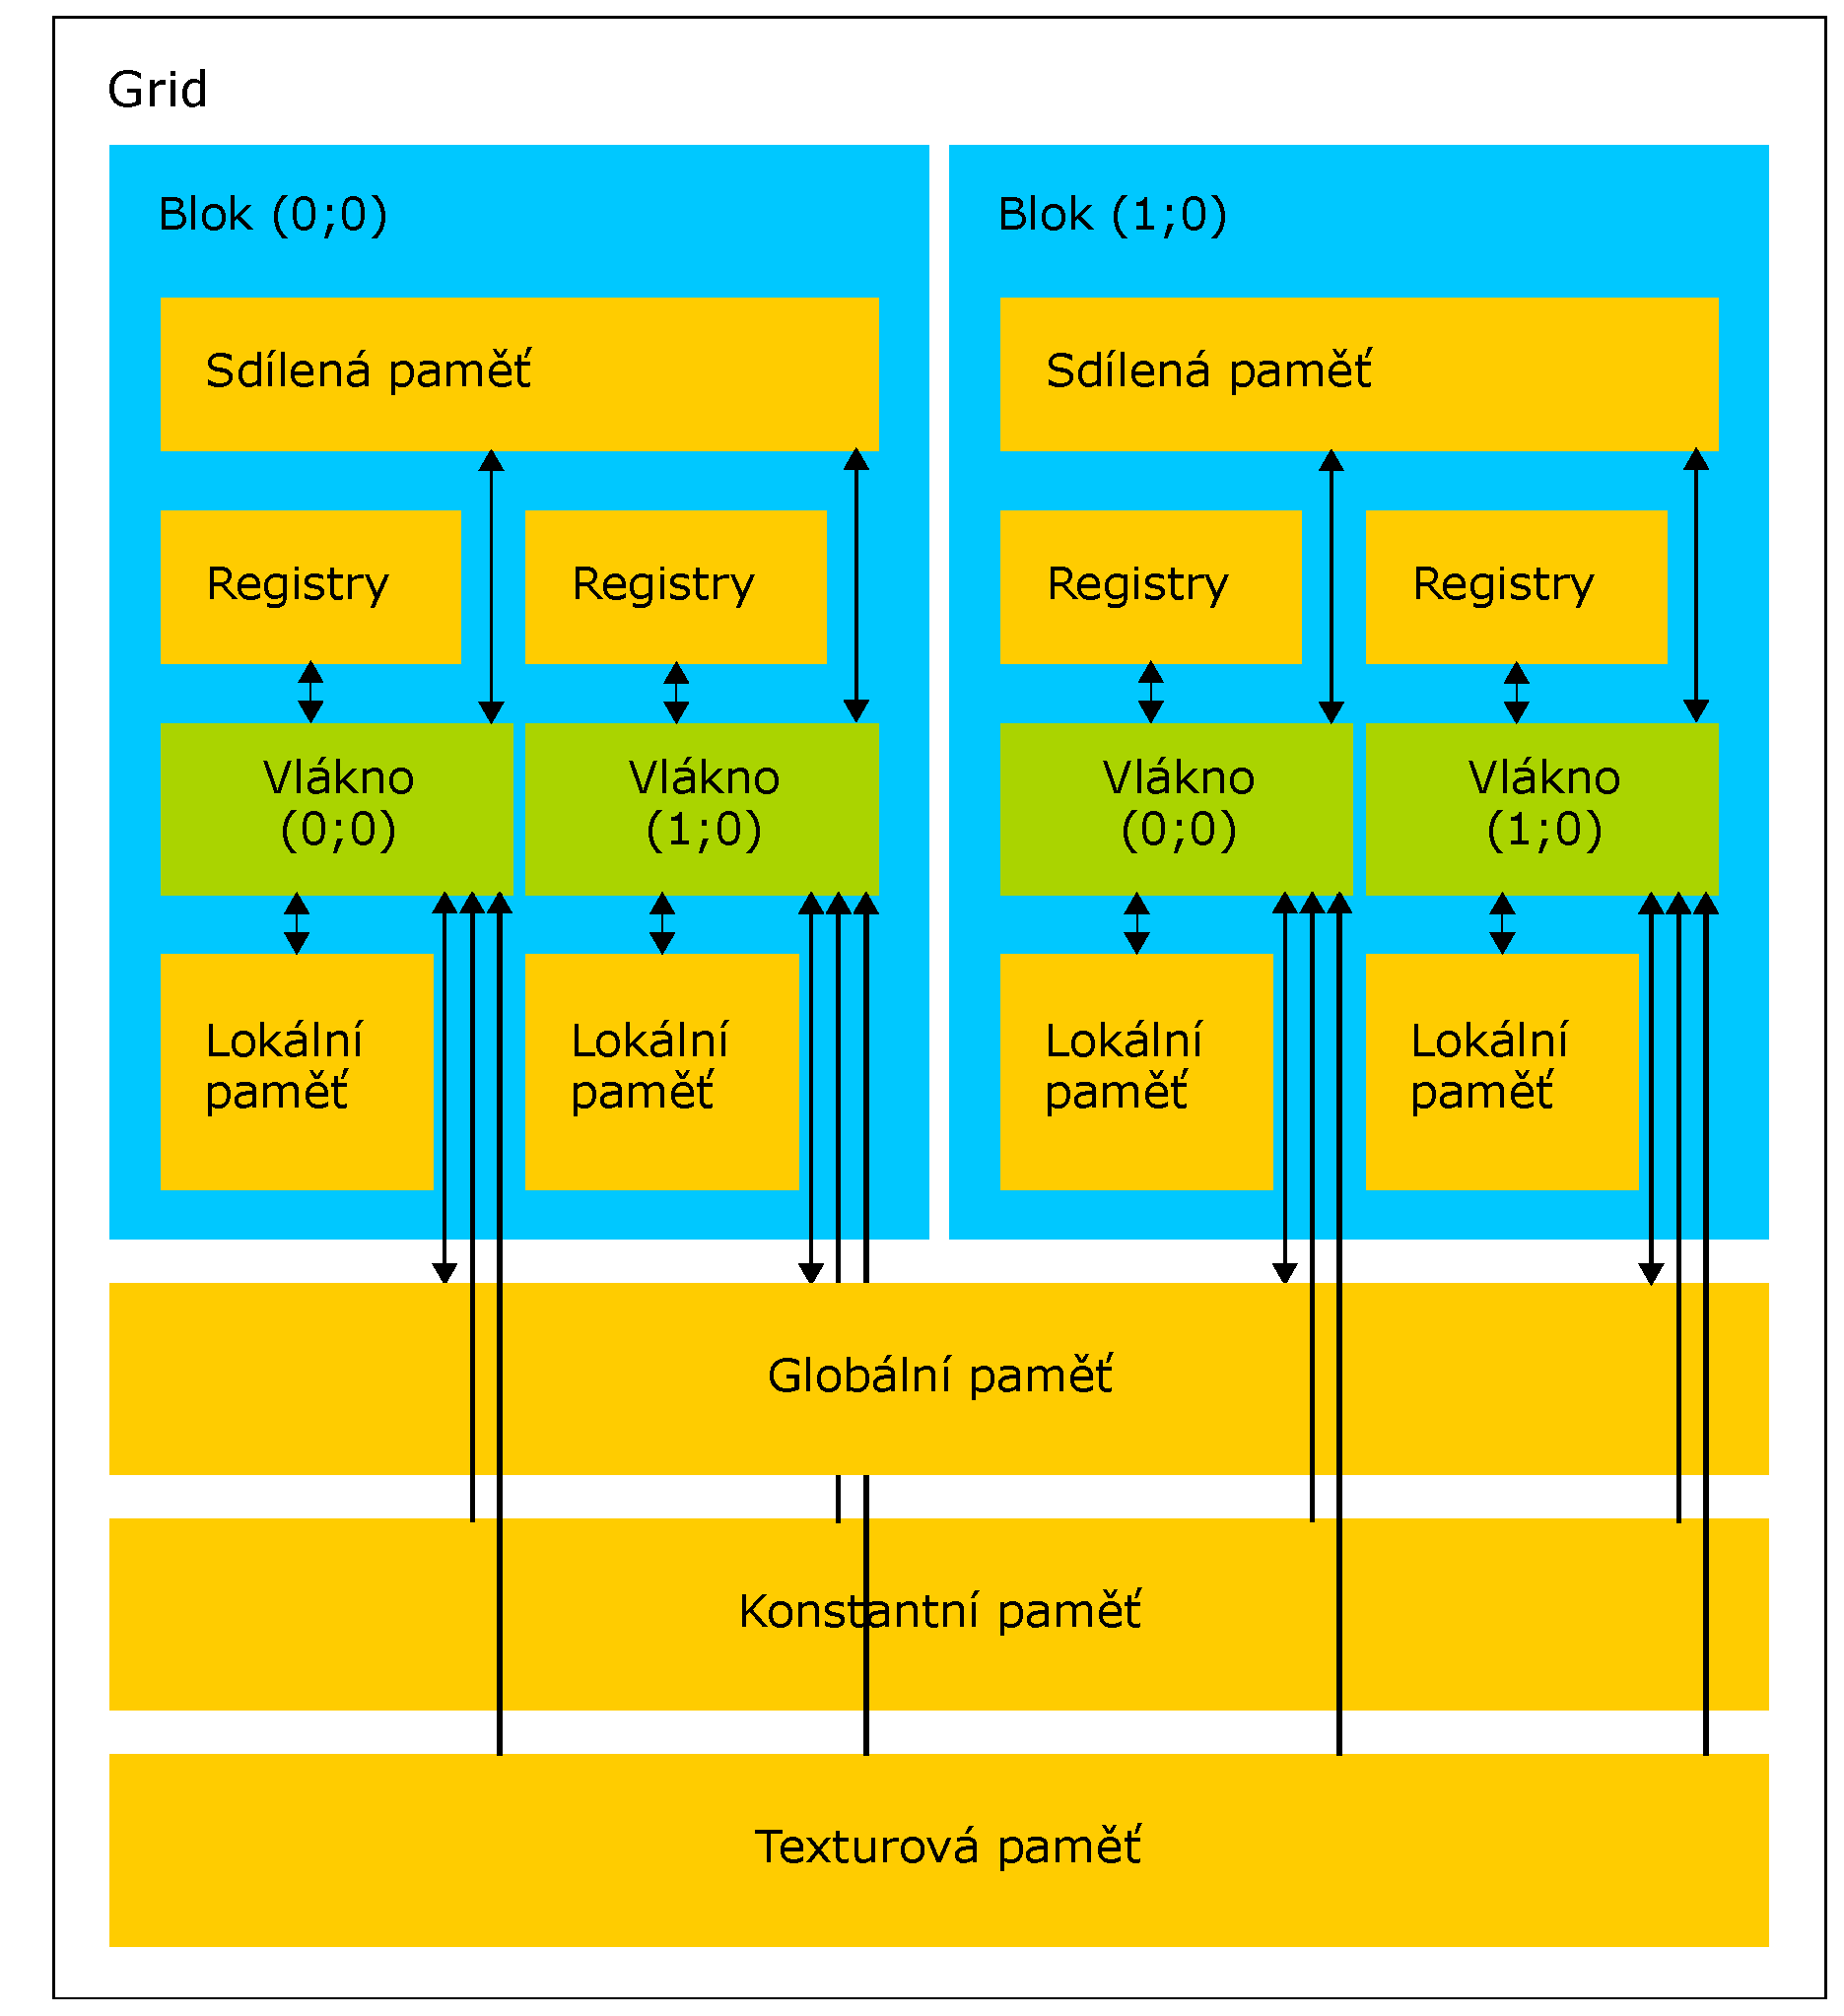
\includegraphics[width=0.6\linewidth]{img/CUDAmemAccess.eps}
  \caption{CUDA Memory access}
  \label{fig:cudamemaccess}
\end{figure}

\begin{description}
\item[Global memory] it is the largest memory (GBs) and it has high bandwidth (usually around 100 GBps) but high latency (400-600 clock cycles). It could be allocated eithe as CUDA arrays or as linear memory. CUDA arrays are opaque memory layouts optimized for texture catching. Linear memory exists on device in a 40-bit address space, so separately allocated entities ca reference another via pointers.~\cite{CUDAGuide} It is used for storing data transfered from host memory and it is allocated and released in host code by special CUDA API function before kernel launch. Global memory allocation is independent on kernel (except dynamically allocated memory inside kernel) and it could be used in many kernels without releasing and allocating new one for other kernel. Memory transfers are special host code CUDA API functions too, but they could be asynchronous. Same as memory allocation/deallocation, data are persistent between one kernel end and other kernel start. When data from this memory are accessed, they are cached in L2 cache. Also processed data or output is stored here before it is transfered back to host. It is operated in transactions of 32B - 128B so for better performance it is better to access data aligned on transaction size. Physically, it is off the chip, but on the device.

\item[Shared memory] is memory shared by all threads running on same SM. Shared memory has lower latency than global memory (32 bits / 2 cycles on CC 1.x and 2.x and 64 bits / 1 cycle on 3.x) than Global memory, but it is also smaller (depend on Compute Capability, from 16 kB on 1.x CC to 48kB on 2.x CC and 3.x CC). It could be as fast as registers if there are no bank conflicts. Shared memory has read-after write dependency which takes 24 clock cycles, but could be hidden by enough active warps. In shared memory are stored statically allocated variable or dynamic memory block could be allocated on kernel launch (it is one of kernel function parameters) and data are copied from global memory in kernel execution. Releasing of memory is done automatically after kernel is finished, so data stored here are not persistent between two kernels, they are even no persistent between same kernel re-execution.\\
This memory is divided into banks, each bank could be accessed independently which is really fast but if there are conflicts in accessing to same bank from multiple threads, access to the bank is serialized (except reading same address which is called broadcast) and could be many times slower, so for the best performance, it is better to avoid these conflicts (for example when threads accessing banks linearly~\ref{fig:linearaccess} or with stride~\ref{fig:strideaccess}, which is not a divisor of total banks count). On CC 1.x and CC 2.x, bank size is 32 bits, on CC 3.0 we can select between 32 bits and 64 bit banks. Physically it is situated near each processor for fast access.\\
\end{description}

\begin{figure}[h]
\centering
\begin{subfigure}{1.0\textwidth}
  \centering
  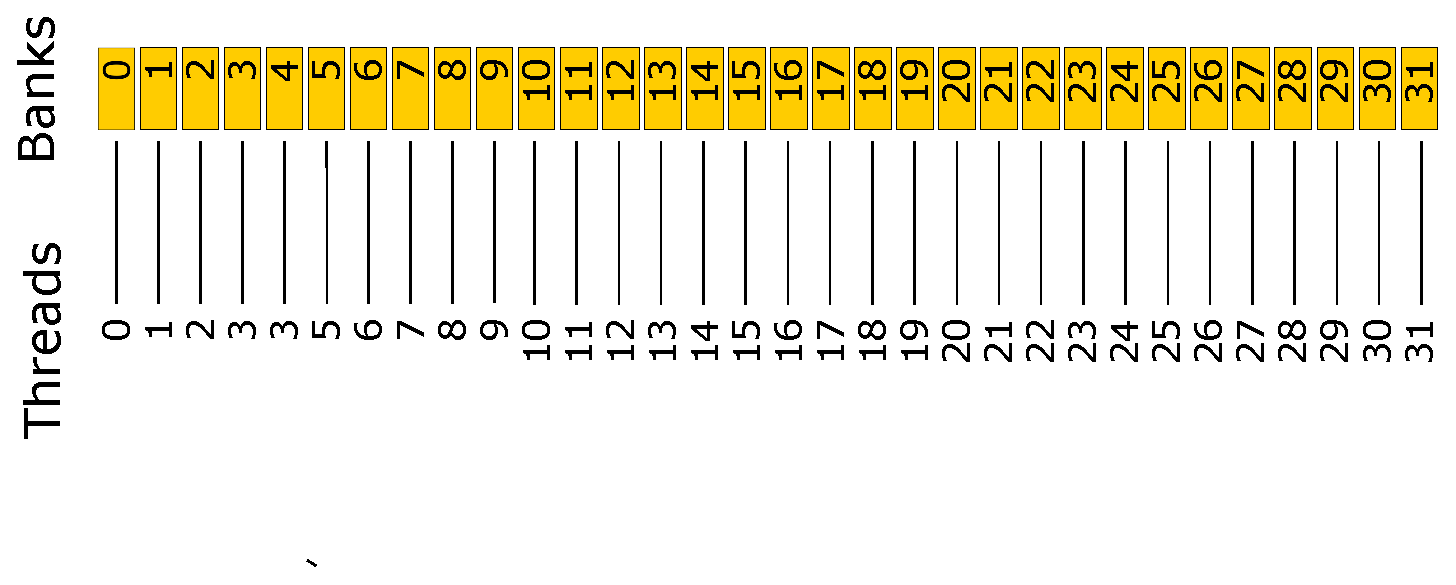
\includegraphics[width=.9\linewidth]{img/sharedMemoryLinearAccess.eps}
  \caption{Linear Access to shared memory}
  \label{fig:linearaccess}
\end{subfigure}
\begin{subfigure}{1.0\textwidth}
  \centering
  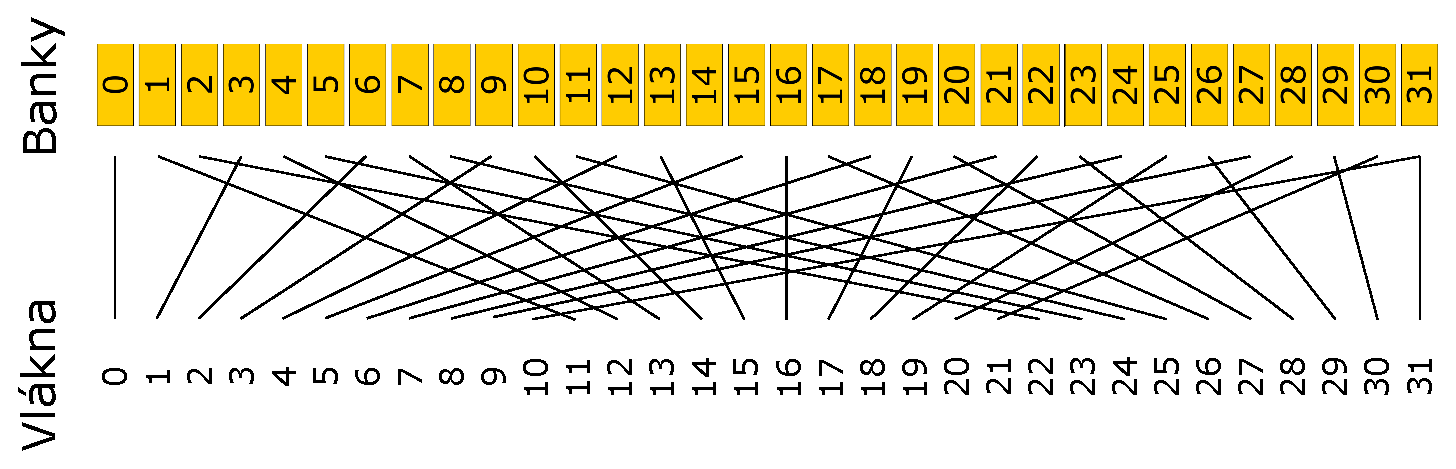
\includegraphics[width=.9\linewidth]{img/sharedMemoryStrideAccess.eps}
  \caption{Access to Shared Memory with stride 3}
  \label{fig:strideaccess}
\end{subfigure}
\caption{Shared Memory access}
\end{figure}

\begin{description}
\item[L1 Cache] has on most devices similar parameters as Share memory, because it has same resource. L1 cache is used for caching accesses to local and global memory so it could significantly speed up the memory access (100x-150x). We can configure which memory should be preferred and bigger by special CUDA API function from host code. On CC 5.0, L1 cache was merged with texture cache and is independent on shared memory (resources are not shared).
\item[Registers] Each multiprocessor has own register pool. Depend on CC, it has 8-64k of 32-bit registers. registers are the smallest memory, but also has the smallest latency (they are as fast as cores). For programmer, registers are not directly controllable. Only slow down is read-after write dependency, same as Shared memory, which takes 24 clock cycles, but it could be also hidden by enough of active warps. If kernel uses more registers than available, registers are stored to local memory. This problem is called \textit{registry spilling}.\\
Each thread has the same amount of registers. The number of registers per thread and the number of blocks determines, how many blocks could reside on SMP. For example, on CC 2.x, if kernel uses 32 registers and each block contains 512 threads, than two blocks can reside on SMP since they require $2*512*32$ registers, which exactly matches the number of registers available on SMP. If kernel uses one more register, than only single block could reside on SMP~\cite{CUDAGuide}.
\item[Local memory] is memory reserved in Global memory accessible by a single thread only. Only some automatic variables are stored in local memory~\cite{CUDAGuide}:
\begin{itemize}
\item Arrays for which it cannot determine that they are indexed with constant quantities,
\item Large structures or arrays that would consume too much register space,
\item Any variable if the kernel uses more registers than available (this is also known as register spilling).
\end{itemize}
Access to local memory are always cached by L1 and L2 memory on CC 2.x and CC 3.x. On CC 5.x, local memory accesses are always stored in L2 cache. 

\item[Constant memory] is a special memory for read-only data. Its size is 64kB and from CC 2.x, compiler stores here constant, thread-independent variables. From CC 2.x, compiler is forced to loading all constant, thread independent variables into this cache.
\item[Texture memory] is special memory used for graphics. Its benefit is 2D spatial locality used mainly for textures.
\end{description}

Data transfer between host and device are much slower than on device memory transfers (the limitation of PCI Express is 16/32 GBps depend on version, but could be slowed by host memory if the host memory is not fast enough or if source memory is swapped on disk). Memory transfer also take significant overhead, which could make CUDA inefficient for small data and compute inexpensive tasks. This problem could be solved by bulk transfers instead of individual memory transfers. Data transfer could be hidden by overlapping data transfer with computing, because CUDA device is capable of computing and simultaneously perform two asynchronous data transfers so for example, input data could be transfer for next computation step, kernel run and results from previous step could be transfered to host at one moment.\\
The host memory could be \textit{pinned} (or page locked) which could speed up memory transfer on systems with front side bus. \textit{Pinned memory} could be also used for \textit{Mapped memory} which allows eliminating memory transfers by mapping host memory into address space of device. All data transfers are than implicitly performed when data are needed by the kernel.

% is little bit different, because programmer can split execution of instructions into different branches by conditions based on thread identification. In both models